% --- A R C H I T E K T U R M O D E L L I E R U N G ---

Wie in Unterkapitel \ref{Allgemeines} bereits ausführlich beschrieben wurde, zählt die effiziente Umsetzung funktionaler und nicht-funktionaler Anforderungen des Auftraggebers zu den wichtigsten Zielen der Softwarearchitektur. Diese Anforderungen werden in Unterkapitel \ref{Anforderungsanalyse} näher erläutert. Basierend auf den Ergebnissen der Anforderungsanalyse wird ein Architekturstil ausgewählt, wobei eine Auswahl moderner Architekturstile in Unterkapitel \ref{Architekturstile} näher beschrieben wird. Darüber hinaus sind weitere Entscheidungen zu treffen, wie die Wahl der Technologien, die Unterteilung des Systems in kleinere, verwaltbare Teile und andere relevante Aspekte.

Dieser Prozess wird in regelmäßigen Abständen wiederholt, um anhand von Feedback und neuen Erkenntnissen, die während der Entwicklung gewonnen werden, Anpassungen vorzunehmen und die Architektur der Software kontinuierlich zu verbessern.

Bevor mit der Implementierung der Software begonnen wird, ist es essenziell, dass ein erster Entwurf der Architektur vorliegt.
Eine gute Planung bietet den Projektteammitglieder nicht nur eine klare Orientierungshilfe, sondern hilft auch, potenzielle Herausforderungen frühzeitig zu erkennen.
\cite{EA:Web15, EA:Web16}


% --- A R C H I T E K T U R M O D E L L I E R U N G ---

\subsection{Architekturmodellierung} \label{Architekturmodellierung}

    Wie in Abschnitt \ref{Die Rolle von Softwarearchitekt/innen} beschrieben, muss der/die Softwarearchitekt/in in der Lage sein, das Projektteam in eine bestimmte Richtung zu lenken. Dabei ist es wichtig, dass alle Teammitglieder sowohl die funktionalen als auch die nicht-funktionalen Anforderungen des Projekts kennen und zumindest einen groben Überblick über die zugrundeliegende Softwarearchitektur haben.

    Da die Architektur eines Softwaresystems sehr komplex und umfangreich sein kann, können \textbf{Visualisierungstechniken} eingesetzt werden, um die \textbf{Komplexität zu reduzieren}. Dies bezeichnet man als Architekturmodellierung, bei der die wesentlichen Eigenschaften des Systems identifiziert und dargestellt werden, um das System besser zu verstehen. 
    
    Das Ziel ist es, einen klaren Überblick zu schaffen und fundierte Entscheidungen anhand dieser Darstellungen zu treffen.
    Nicht nur das Projektteam profitiert davon, sondern auch neue Teammitglieder, die so schneller ins Projekt integriert werden können.

    Es gibt zahlreiche Tools und Standards, die für die Visualisierung der Softwarearchitektur verwendet werden können.
    Im Folgenden werden zwei der bekanntesten Modellierungstechniken näher beschrieben.
    \cite{EA:Web12, EA:Web13, EA:Web14}


     % --- U N I F I E D   M O D E L I N G   L A N G U A G E   ( U M L ) ---

    \subsubsection{Unified Modeling Language (UML)} \label{UML}

    Die Unified Modeling Language (UML) ist eine standardisierte Modellierungssprache, die verwendet wird, um bestimmte Teile eines Softwaresystems grafisch darzustellen.

    Durch den Einsatz von UML können Diagramme erstellt werden, die als Kommunikationsmittel zwischen unterschiedlichen Stakeholdern genutzt werden können. \\
    Diese Diagramme bieten den Vorteil, dass sie auch von Personen verstanden werden können, die keine Programmierkenntnisse besitzen und komplexe Systeme einfach darstellen.
    \cite{EA:Web18, EA:Web19}

    Es gibt 14 offiziell anerkannte Arten von UML-Diagrammen, die in \textbf{zwei Kategorien} unterteilt werden:
    \begin{itemize}
        \item Strukturelle Diagramme
        \item Verhaltensdiagramme
    \end{itemize}

    In Abbildung \ref{fig:uml-diagrams} sind die verschiedenen UML-Diagrammtypen dargestellt:

    \begin{figure}[H]
        \centering
        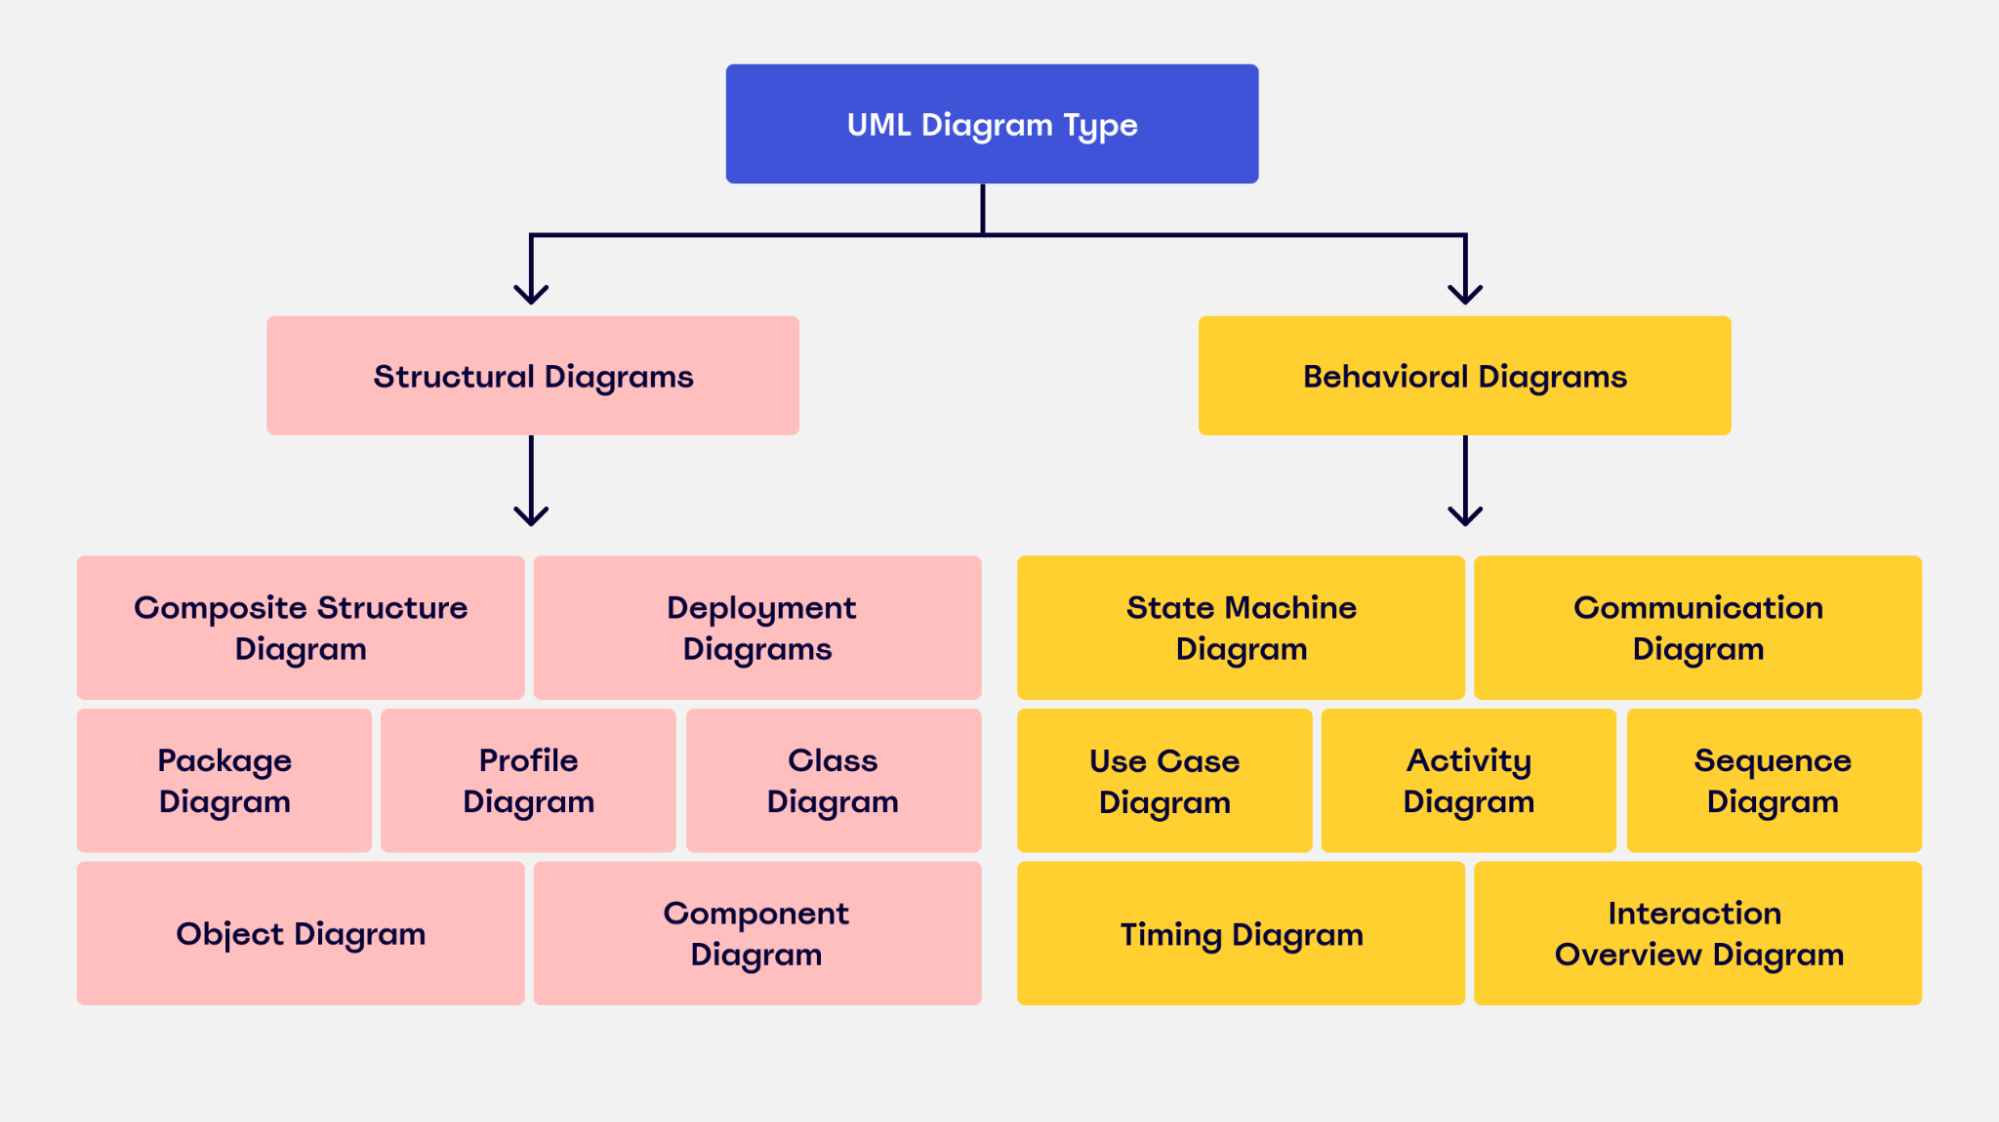
\includegraphics[width=1\linewidth]{images//EA/uml-diagrams.png}
        \caption{Arten von UML-Diagrammen \\ \cite{EA:Web17}}
        \label{fig:uml-diagrams}
    \end{figure}

    \clearpage

    Da es den Rahmen dieser Arbeit sprengen würde, jeden einzelnen UML-Diagrammtyp im Detail zu erklären, wird die allgemeine Unterscheidung zwischen Struktur- und Verhaltensdiagrammen betrachtet. Anschließend wird jeweils ein Struktur- und ein Verhaltensdiagramm näher beschrieben, die in der Praxis besonders häufig Anwendung finden und in Bezug auf das Projekt \textbf{CGM MAXX LITE} von Bedeutung sind.


    % --- S T R U K T U R E L L E   D I A G R A M M E ---

    \textbf{Strukturelle Diagramme} veranschaulichen den \textbf{Aufbau eines Softwaresystems} oder einzelner Teile davon. 
    Dabei werden Komponenten wie Klassen, Objekte und Module sowie deren Beziehungen dargestellt, die für die Struktur der Software entscheidend sind.


        % --- K L A S S E N D I A G R A M M ---

        Das bekannteste Strukturdiagramm ist das \textbf{Klassendiagramm}, wobei das System, oder nur ein Teil davon, durch Klassen abgebildet wird.
        Jede Klasse hat dabei bestimmte Attribute (Daten) und Methoden (Funktionen), die für unterschiedliche Aufgaben genutzt werden können.
        \cite{EA:Web17, EA:Web18}
    
        Ein Beispiel für ein Klassendiagramm ist in Abbildung \ref{fig:class-diagram-file-upload} zu finden.
        Es zeigt die Klassen, die im Rahmen des Projekts CGM MAXX LITE für den File-Upload erforderlich sind.
    
        Hierbei handelt es sich um die \textbf{Klassen einer Spring-Boot-Applikation}. Da diese Anwendung neben dem Hochladen von Dateien auch noch weitere Funktionalitäten bietet, konzentriert sich dieses Diagramm \textbf{nur} auf die \textbf{Klassen, die für das Hochladen von Dateien relevant sind}. 
        Dadurch wird ein besserer Überblick gewährleistet und es ist einfacher das Diagramm zu verstehen, ohne sich von irrelevanten Klassen oder Methoden ablenken zu lassen.
    
        Hier eine kurze Erklärung der wichtigsten Klassen:
        \begin{itemize}
            \item \lstinline{FileUploadController} ... RESTful-Controller, der die Schnittstellen für die Kommunikation zwischen Frontend und Backend bereitstellt.
            
            \item \lstinline{FileUploadServiceImpl} ... Service, der die gesamte Business-Logik umfasst. Dazu gehört nicht nur das Speichern von Fotos und Audioaufnahmen, sondern auch die richtige Benennung dieser Dateien.
            
            \item \lstinline{FileInfoService} ... wird verwendet, um die Anzahl der Dateien zu ermitteln, die an einem bestimmten Tag für einen bestimmten Patienten hochgeladen wurden. Dies ist notwendig für eine einheitliche Benennung der Dateien.
            
            \item \lstinline{PatientService} ... überprüft, ob der/die Patient/in, für den eine Datei hochgeladen werden soll, existiert.
            
            \item \lstinline{FileRepository} ... verwaltet \lstinline{File}-Entitäten (CRUD\footnote{Abkürzung für Create, Read, Update und Delete}-Operationen)
        \end{itemize}
    
        \begin{figure}[H]
            \centering
            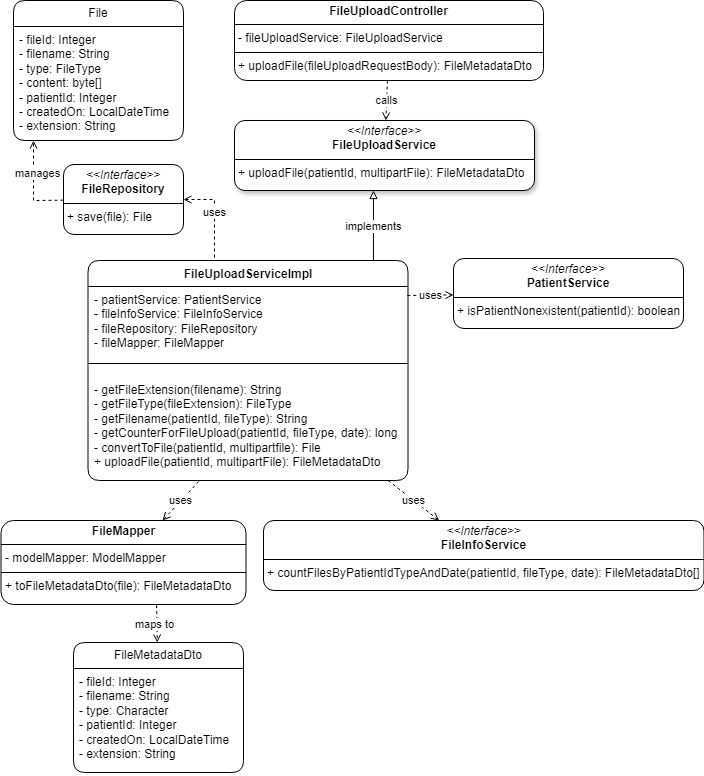
\includegraphics[width=1\linewidth]{images/EA/uml-class-diagram.png}
            \caption{Klassendiagramm - File Upload im Projekt CGM MAXX LITE}
            \label{fig:class-diagram-file-upload}
        \end{figure}

        Neben den Klassen in Abbildung \ref{fig:class-diagram-file-upload} sind auch die Beziehungen zwischen diesen durch unterschiedliche Pfeile gekennzeichnet, die durch das Hinzufügen von Beschriftungen noch leichter nachvollzogen werden können.

        \clearpage

        Im oben abgebildeten Klassendiagramm kommen nur zwei Arten von Beziehungen zum Einsatz:
        \begin{itemize}
            \item Vererbung (Inheritance)
            \item Abhängigkeit (Dependency)
        \end{itemize}

        Dabei implementiert \lstinline{FileUploadServiceImpl} das Interface \lstinline{FileUploadSerive}. Die restlichen Beziehungen zeigen Abhängigkeiten, bei denen bestimmte Klassen mithilfe von \textbf{Dependency Injection\footnote{Technik, bei der Objekte ihre Abhängigkeiten von anderen Objekten erhalten \cite{EA:Web22}}} eingebunden werden, um bestimmte Methoden aufzurufen. 
        \cite{EA:Web21}

        Auf den ersten Blick wirkt das Diagramm möglicherweise etwas komplex, betrachtet man es jedoch genauer, erkannt man, dass es \textbf{nach außen hin nur eine Schnittstelle} gibt, auf die zugegriffen werden kann. Im Folgenden wird gezeigt, wie auf die Schnittstelle zugegriffen werden kann. \\
    
       \lstinputlisting[
            caption=\texttt{FileUploadController.java},
            label=lst:file-upload,
            firstline=10
        ]{sources/EA/FileUploadController.java}
    
        Der in \lil{lst:file-upload} definierte REST-Controller ermöglicht das Hochladen einer Datei für eine/n Patient/in über einen \textbf{POST-Request}. Dabei wird der \\ \lstinline{FileUploadService} aufgerufen, um die Datei korrekt zu benennen und anschließend in der Datenbank zu speichern.

        \clearpage
    
        % --- V E R H A L T E N S D I A G R A M M E ---

        Neben strukturellen Diagrammen gibt es auch \textbf{Verhaltensdiagramme}.
        Diese stellen das dynamische Verhalten eines Systems dar.
        Dabei spielt nicht nur das Geschehen innerhalb des Systems eine Rolle, sondern auch wie das System mit anderen Systemen und Benutzern interagiert. Verhaltensdiagramme eignen sich deshalb besonders gut, um \textbf{Abläufe und Geschäftsprozesse} zu \textbf{visualisieren}.
        \cite{EA:Web18, EA:Web20}

        Um ein Diagramm zu erstellen, das nicht nur die Struktur der Klassen darstellt, sondern auch erklärt, in welcher Reihenfolge bestimmte Interaktionen erfolgen, kann ein sogenanntes \textbf{Sequenzdiagramm} verwendet werden. Dies ermöglicht es, den genauen Ablauf eines bestimmten Prozesses nachzuvollziehen.
        \cite{EA:Web23, EA:Web24} \\

        \begin{figure}[H]
            \centering
            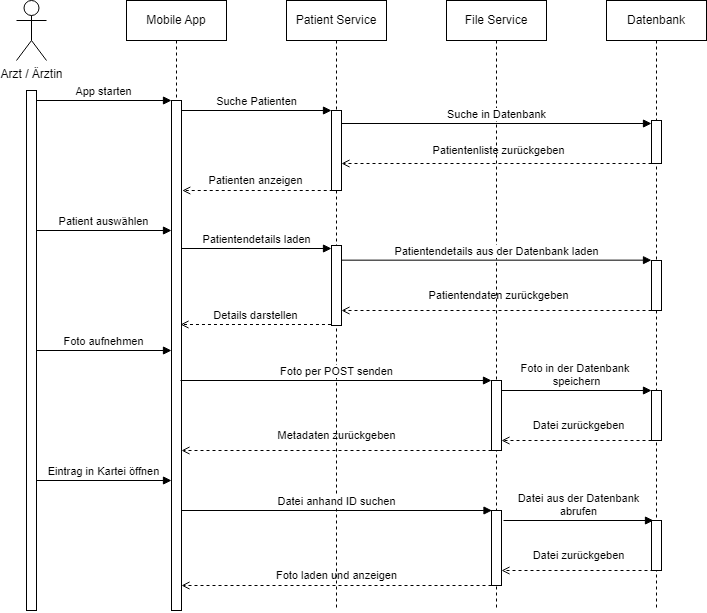
\includegraphics[width=1\linewidth]{images/EA/uml-sequence-diagram.png}
            \caption{Sequenzdiagramm - File Upload im Projekt CGM MAXX LITE}
            \label{fig:sequence-diagram-file-upload}
        \end{figure}

        \clearpage

        Um den Unterschied zwischen strukturellen Diagrammen und Verhaltensdiagrammen zu verdeutlichen, stellt das Sequenzdiagramm in Abbildung \ref{fig:sequence-diagram-file-upload} ebenfalls den File-Upload dar. Während das Klassendiagramm in Abbildung \ref{fig:class-diagram-file-upload} die Struktur der Klassen beschreibt und einen Bezug zum Code herstellt, zeigt das Sequenzdiagramm die notwendigen Schritte, um eine Datei in der Datenbank abzulegen und später in der App abzurufen.

        Folgende Elemente werden im Sequenzdiagramm \ref{fig:sequence-diagram-file-upload} verwendet:
        \begin{itemize}
            \item Akteur/innen
            \item Objekte
            \item Lebenslinien
            \item Aktivitätsbalken
            \item Synchrone Nachrichten (durchgezogene Linie mit ausgefüllter Spitze)
            \item Asynchrone Antworten (strichlierte Linie mit offener Spitze)
        \end{itemize}

        Im Folgenden wird der Ablauf des Sequenzdiagramms näher beschrieben, um den Einsatz und die Bedeutung der einzelnen Elemente zu erklären. \cite{EA:Web24}

        Da die Software CGM MAXX LITE hauptsächlich von \textbf{Ärzten/innen} verwendet wird, gibt es hier \textbf{nur einen Akteur/eine Akteurin}. Akteur/innen sind also Entitäten, die mit dem System interagieren. Die \textbf{Objekte} stellen \textbf{einzelne Teile des Systems} dar.
        Dieses besteht aus einer mobilen Benutzeroberfläche, einer zentralen Datenbank und zwei Microservices. Der eine Microservice ist verantwortlich für die Patientenverwaltung, das andere kümmert sich um die Verwaltung von Fotos und Audioaufnahmen. Die \textbf{strichlierten Linien unterhalb der Objekte} stellen deren \textbf{Lebenslinien} dar. Die \textbf{darüberliegenden Balken} bezeichnet man als \textbf{Aktivitätsbalken}. Diese stellen dar, wann auf bestimmte Objekte zugegriffen wird.
        Was genau passiert, wird durch \textbf{verschiedene Pfeile und kurze Beschreibungen} dargestellt.
        Die Akteur/innen können dabei nur auf die mobile Applikation zugreifen, die im Hintergrund auf die einzelnen Services zugreift. 

        Möchte ein Arzt oder eine Ärztin ein Foto hochladen, werden zunächst die Patient/innen aus der Datenbank geladen. Anschließend kann der/die gewünschte Patient/in ausgewählt werden. Dabei wird die Detailansicht geöffnet und es kann ein Foto aufgenommen werden. Ein POST-Request wird an den File Service gesendet, der das Foto verarbeitet, benennt es korrekt, in der Datenbank speichert und  anschließend die Metadaten der hochgeladenen Datei zurückgibt, um zu bestätigen, dass der Upload erfolgreich war.
        
        \clearpage
    

    % --- C 4 - M O D E L L ---

    \subsubsection{C4-Modell}

    Neben UML gibt es zahlreiche weitere Methoden, um die Architektur einer Software zu modellieren.
    Eine davon ist das \textbf{C4-Modell}, dessen Name für \textbf{Context, Containers, Components und Code} steht.
    Ähnlich wie UML zielt auch das C4-Modell darauf ab, das Verständnis unterschiedlicher Interessensgruppen zu verbessern, um eine Grundlage für erfolgreiche Projektergebnisse zu schaffen. Dabei wird das \textbf{System in vier Ebenen dargestellt}. 
    \cite{EA:Web25, EA:Web26, EA:Web28}

    Als nächstes werden die einzelnen Ebenen näher beschrieben:

    Die \textbf{erste Ebene} bezieht sich auf den \textbf{Systemkontext}. Bei einem Systemkontext-Diagramm liegt der Fokus darauf, 
    einen \textbf{groben Überblick über das System} zu schaffen, ohne näher auf spezifische Technologien und technische Details einzugehen.
    Genauer gesagt beschreibt es, wofür das System zuständig ist, von wem es verwendet wird und wie es mit anderen Systemen interagiert.
    Solche Diagramme eignen sich besonders gut, um mit nicht-technischen Stakeholdern zu kommunizieren.
    \cite{EA:Web27}

    In Abbildung \ref{fig:c4-system-context-diagram} wird das Systemkontext-Diagramm für das Projekt CGM MAXX LITE dargestellt:

    \begin{figure}[H]
        \centering
        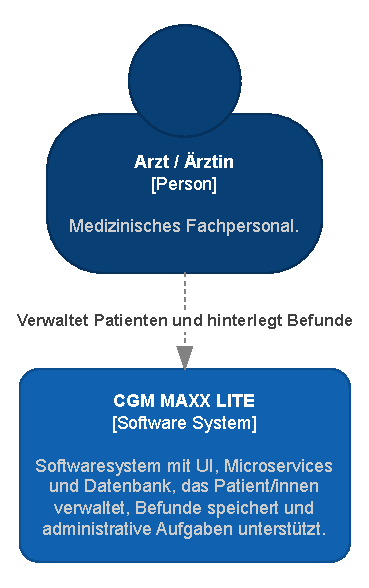
\includegraphics[scale=1.05]{pdf/EA/c4-system-context-diagram.pdf}
        \caption{Systemkontext-Diagramm - CGM MAXX LITE}
        \label{fig:c4-system-context-diagram}
    \end{figure}

    \clearpage

    Die \textbf{zweite Ebene} stellt die \textbf{einzelnen Container eines Systems} dar. Container stellen die grundlegenden Bestandteile eines Systems dar, die unabhängig voneinander gestartet, bereitgestellt und betrieben werden können.
    \textbf{Container-Diagramme} zeigen zusätzlich auch die verwendeten Technologien und wie die Container miteinander kommunizieren. 
    Sie können eingesetzt werden, um \textbf{Softwareentwickler/innen bei der Entwicklung zu unterstützen}. Das bietet den Vorteil, dass Abhängigkeiten zwischen Container einfacher nachvollzogen werden können. 
    \cite{EA:Web28}
    
    \begin{figure}[H]
        \centering
        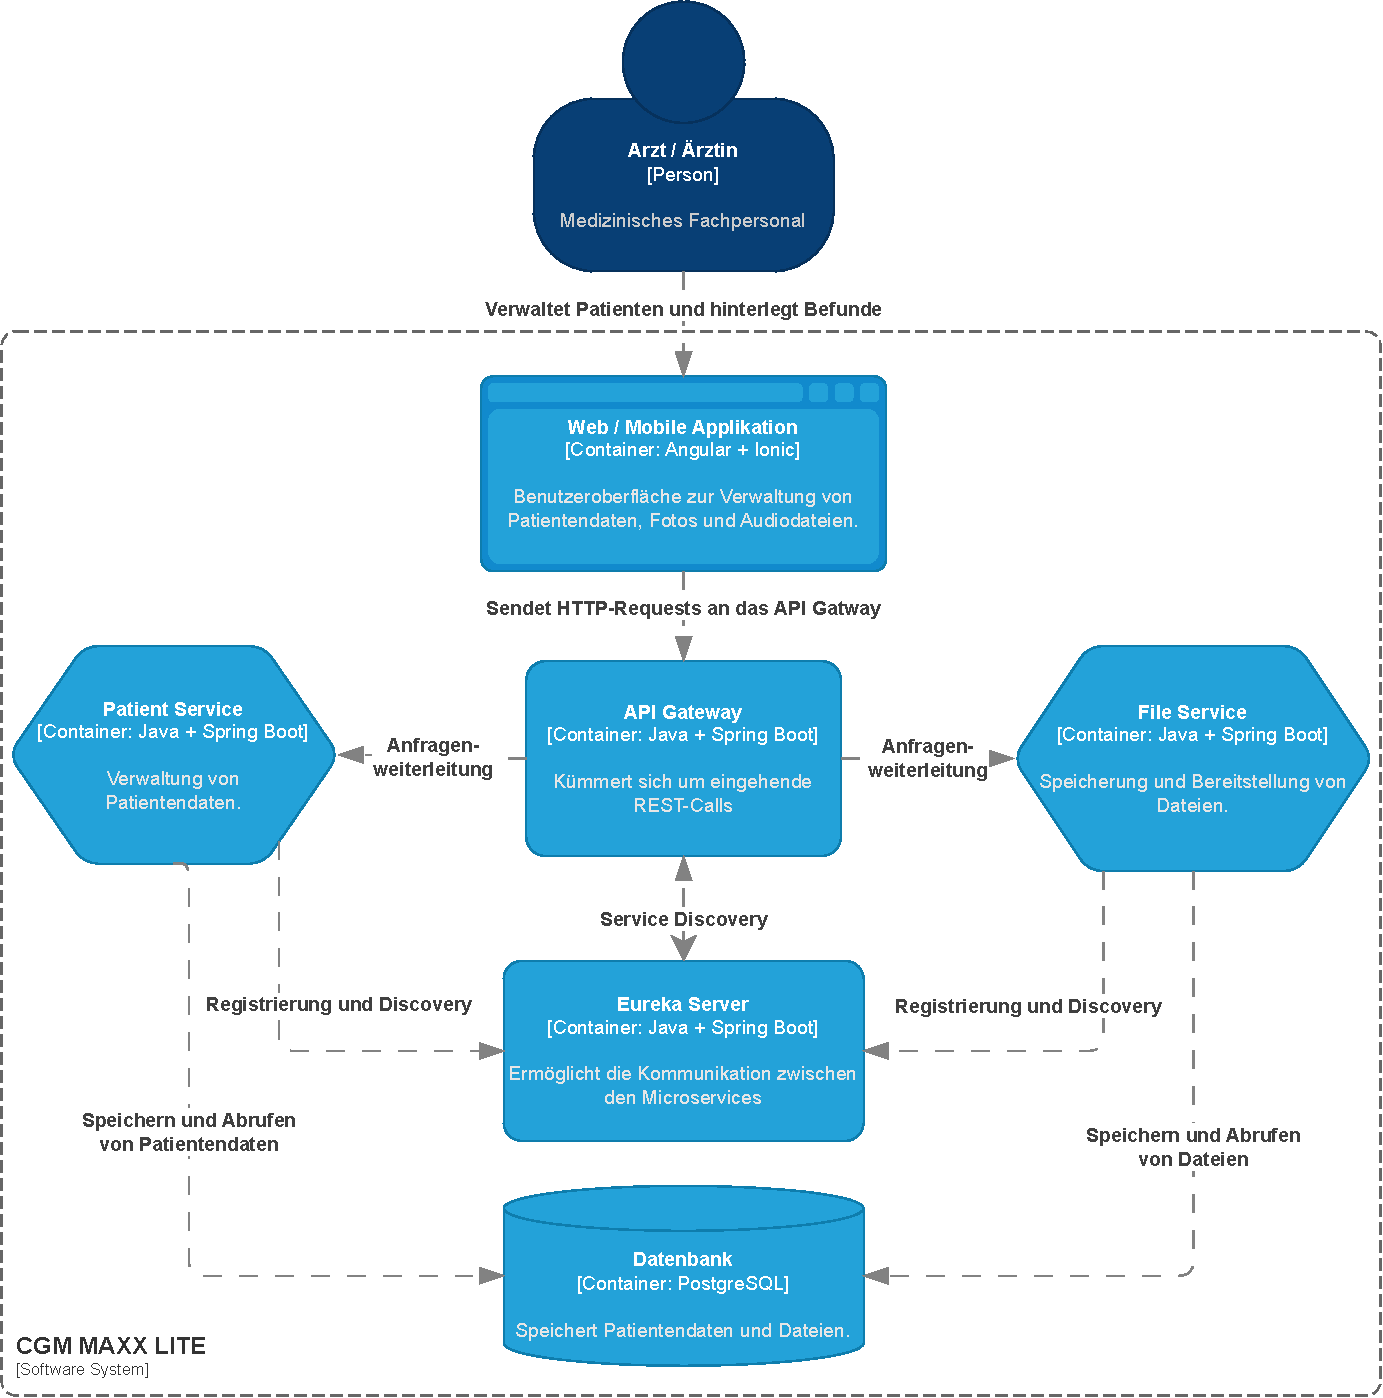
\includegraphics[scale=0.7]{pdf/EA/c4-container-diagram.pdf}
        \caption{Container-Diagramm - CGM MAXX LITE}
        \label{fig:c4-container-diagram}
    \end{figure}

    In Abbildung \ref{fig:c4-container-diagram} wird ein Container-Diagramm dargestellt, das die wichtigsten Bestandteile des Projekts CGM MAXX LITE zeigt. 
    
    Dabei gibt es unterschiedliche Arten von Containern:
    \begin{itemize}
        \item Web-App / Mobile App
        \item API-Gateway
        \item Microservices
        \item Service Discovery Server
        \item Datenbank
    \end{itemize}

    Eine genaue Beschreibung der einzelnen Container ist in Abschnitt \ref{Projektbezug - Architekturstil} zu finden.

    Da es zu umfangreich wäre, für jede Ebene des C4-Modells ein spezifisches Diagramm für CGM MAXX LITE zu erstellen, und es zudem schwierig ist, alle Komponenten auf einer Seite darzustellen, werden die folgenden Ebenen ausschließlich textlich beschrieben.

    Die \textbf{dritte Ebene} ermöglicht einen genaueren Blick auf die \textbf{Elemente innerhalb eines Containers}.
    Mithilfe eines \textbf{Komponentendiagramms} kann dargestellt werden, welche Aufgaben die einzelnen Komponenten erledigen, wie sie miteinander interagieren und welche Technologien oder Implementierungen dabei zum Einsatz kommen.
    \cite{EA:Web27, EA:Web28}

    Ein Beispiel für eine Komponente ist ein REST-Controller in Spring Boot. Bezieht man sich dabei auf das Projekt, so wäre die Java-Klasse \textbf{FileUploadController.java} in \lil{lst:file-upload} eine Komponente.

    Die \textbf{vierte} und letzte \textbf{Ebene} des C4-Modells betrachtet die Implementierung einzelner Komponenten.
    Dazu können \textbf{UML-Klassendiagramme} eingesetzt werden. Auch hierfür gibt es bereits ein Beispiel in Abbildung \ref{fig:class-diagram-file-upload}
    Solche Diagramme müssen oft nicht selbst erstellt werden, da sie mithilfe von IDEs\footnote{Integrierte Entwicklungsumgebung} automatisch erstellt werden können.
    \cite{EA:Web28}

    \clearpage

    \subsubsection{Überleitung}
    
    Bevor mit dem nächsten Thema fortgesetzt wird, hier eine kurze Zusammenfassung der wichtigsten Erkenntnisse:
    
    Es gibt unzählige verschiedene Möglichkeiten, um die Architektur einer Software grafisch darzustellen. 
    Diese Visualisierungen können als Kommunikationsmittel eingesetzt werden und helfen dabei, ein besseres Verständnis für das System zu schaffen, unabhängig davon, ob eine Person technische Fähigkeiten besitzt oder nicht. 
    Basierend auf der Zielgruppe können unterschiedliche Diagramme verwendet werden.    
    Je nach Anwendungszweck eigenen sich bestimmte Diagramme besser als andere.
    

% --- C L O U D - S P E Z I F I S C H E   A R C H I T E K T U R E N T S C H E I D U N G E N ---

\subsection{Cloud-spezifische Architekturentscheidungen}

Da der Entwurf einer Software weit mehr als nur die Modellierung betrifft, gibt es einige weitere Entscheidungen, die getroffen werden müssen.
Wie der Name dieser Arbeit bereits verrät, liegt der Fokus auf cloudbasierten Systemen. Neben Planung und Entwicklung muss die Software auch in der Cloud bereitgestellt werden, um sie für die Nutzer/innen zugänglich zu machen.

Damit Anwendungen sicher, zuverlässig und skalierbar in der Cloud bereitgestellt werden können, gibt es \textbf{Entwurfsmuster}, die eingesetzt werden, um bestimmte Probleme der Cloud zu umgehen. Um Software schneller bereitzustellen, kann die Infrastruktur mithilfe von \textbf{Infrastructure as Code} automatisch erstellt werden. \textbf{DevOps und Automatisierung} spielen ebenfalls eine bedeutende Rolle, um Anwendungen einfach bereitzustellen.
\cite{EA:Web30, EA:Web31}

Im weiteren Verlauf wird näher auf diese Themen eingegangen.


    % --- E N T W U R F S M U S T E R   F Ü R   D I E   C L O U D ---

    \subsubsection{Entwurfsmuster für die Cloud} \label{Entwurfsmuster für die Cloud}

    Wie zuvor erwähnt werden Entwurfsmuster eingesetzt, um \textbf{Software zuverlässig in der Cloud zu betreiben}. 
    Vor allem bei verteilten Systemen, bei denen mehrere Komponenten über das Netzwerk miteinander kommunizieren, kann es zu Schwierigkeiten kommen.
    Beispiele dafür sind unzuverlässige Netzwerke, hohe Latenzen oder begrenzte Bandbreiten.

    \clearpage

    Durch den gezielten Einsatz von Entwurfsmustern werden spezifische Probleme zwar nicht beseitigt, aber die Wahrscheinlichkeit, dass diese eintreten, wird dadurch deutlich verringert. Microsoft stellt eine Sammlung von Entwurfsmustern bereit, die auf unterschiedliche Herausforderungen zugeschnitten sind.
    Im Anschluss wird eine Auswahl von Entwurfsmustern beschrieben, die für das Projekt CGM MAXX LITE relevant sind.
    \cite{EA:Web31}

    Ein Entwurfsmuster, das für CGM MAXX LITE von großer Bedeutung ist, heißt \\ \textbf{Backends for Frontends}. 
    Bei diesem Muster wird \textbf{für jede Benutzeroberfläche ein eigenes Backend} erstellt. 

    \begin{figure}[H]
        \centering
        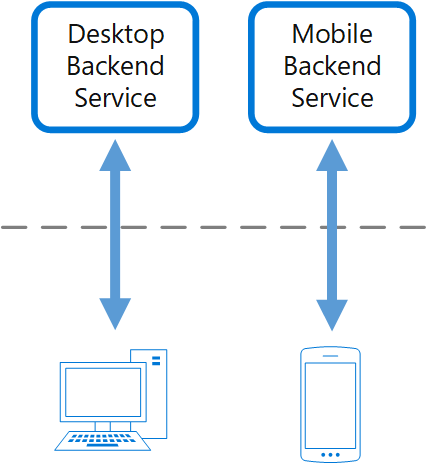
\includegraphics[width=0.45\linewidth]{images/EA/backend-for-frontend.png}
        \caption{Backends for Frontends \\ \cite{EA:Web32}}
        \label{fig:backend-for-frontend}
    \end{figure}

    Wie in Abschnitt \ref{Projektbezug - Anforderungsanalyse} erwähnt, existiert bereits ein Backend für die Desktop-Applikation CGM MAXX. Da diese nicht für den Betrieb auf mobilen Geräten ausgelegt ist, wird im Zuge des Projekts ein Frontend entwickelt, das sich auf mobile Geräte fokussiert. 
    Da die mobile Applikation nur einen Teil der Aufgaben der Desktop-Applikation abdeckt und zusätzlich Funktionen für Kamera und Mikrofon bietet, ist es sinnvoll, ein separates Backend zu entwickeln. So gibt es kein zentrales Backend, das die Anforderungen beider Frontends erfüllen muss, wodurch es zu keinen Konflikten kommen kann. Das bedeutet, dass die Applikationen unabhängig voneinander verändert werden können.
    \cite{EA:Web32}

    \clearpage

    Ein weiteres interessantes Muster ist das \textbf{Compute Resource Consolidation Pattern}.
    Softwaresysteme bestehen oftmals aus mehreren Applikationen, die unabhängig voneinander bereitgestellt werden.
    Dies führt zu einem höheren Bedarf an Computerressourcen, steigenden Bereitstellungskosten und einem größeren Wartungsaufwand. \\

    \begin{figure}[H]
        \centering
        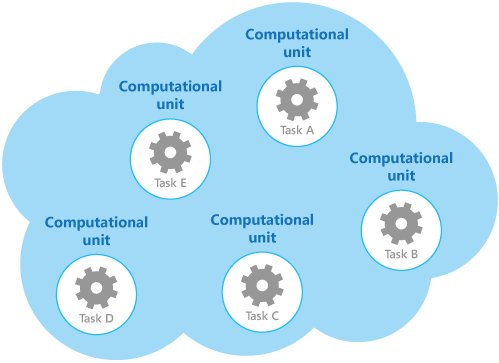
\includegraphics[width=0.55\linewidth]{images/EA/compute-resource-consolidation.png}
        \caption{Vereinfachte Struktur einer cloudbasierten Lösung \\ \cite{EA:Web33}}
        \label{fig:compute-resource-consolidation}
    \end{figure}

    Abbildung \ref{fig:compute-resource-consolidation} zeigt vereinfacht, wie ein verteiltes System in der Cloud aussieht.
    Eine Recheneinheit kann beispielsweise genutzt werden, um ein Microservice zu betreiben.

    In Systemen mit vielen Microservices entstehen jedoch häufig unnötige Kosten, da auf bestimmte Services öfter zugegriffen wird als auf andere. 
    Selbst dann, wenn ein Service gar nicht verwendet wird, entstehen Kosten. Daher ist es wichtig, die Aufteilung der Dienste sorgfältig zu planen, um eine kostengünstige und effiziente Lösung zu schaffen.

    Dieses Muster zielt darauf ab, die \textbf{Auslastung der Recheneinheiten} zu \textbf{erhöhen}, um die \textbf{Kosten für die Ressourcen} zu \textbf{senken}. Erreicht wird dies, indem bestimmte \textbf{Dienste zusammengefasst} und \textbf{auf einer gemeinsamen Recheneinheit betrieben} werden. Außerdem können die Dienste so direkt miteinander kommunizieren, was dazu beiträgt, dass bestimmte Aktionen schneller ausgeführt werden können.

    \textbf{Eingesetzt} wird dieses Muster \textbf{bei Diensten, die die meiste Zeit im Leerlauf verbringen}, um durch das Gruppieren zusammenhängender Einheiten die Kosten zu senken. Weniger geeignet ist für fehlertolerante Vorgänge, da andere Dienste, die auf derselben Recheneinheit betrieben werden, beeinträchtigt werden könnten. \\
    \cite{EA:Web33}

    \clearpage

    Das letzte Entwurfsmuster, das in dieser Arbeit erläutert wird, ist das \textbf{Gateway Routing Pattern}.
    Es kommt zum Einsatz, wenn ein Client innerhalb einer Applikation auf mehrere Dienste zugreift. 
    Dabei fungiert ein \textbf{API-Gateway} als zentraler Kommunikationspunkt, der die \textbf{Anfragen des Clients empfängt} und \textbf{an die entsprechenden Dienste weiterleitet}. Dadurch soll die Komplexität der Kommunikation zwischen dem Client und mehreren Diensten reduziert werden, da der Client nur über einen einzigen Endpunkt mit den Diensten interagiert.
    \cite{EA:Web34}
    
    In Abbildung \ref{fig:gateway-routing} ist das Gateway Routing Pattern dargestellt: 
    
    \begin{figure}[H]
        \centering
        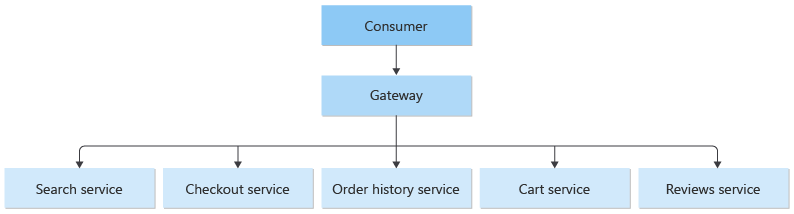
\includegraphics[width=1.05\linewidth]{images/EA/gateway-routing.png}
        \caption{Gatway Routing \\ \cite{EA:Web34}}
        \label{fig:gateway-routing}
    \end{figure}

    Um die Funktionsweise des Musters näher zu verdeutlichen, wird näher auf die Konfiguration des API-Gateways im Projekt CGM MAXX LITE eingegangen. 
    
    In \lil{lst:api-gateway} wird die \textbf{Konfiguration des Gateways} dargestellt:
    \vspace{0.3em}
    \lstinputlisting[
        caption=\texttt{application.yml - API Gateway},
        label=lst:api-gateway,
    ]{sources/EA/application.yml}


    Das API-Gateway lauscht auf den Port 8080 und ermöglicht durch die Definition von Routen den Zugriff auf die dahinterliegenden Microservices. Eine genauere Beschreibung der einzelnen Microservices findet sich in Abschnitt \ref{Projektbezug - Architekturstil}.

     Damit Nutzer/innen diese Services nutzen können, erfolgt der Zugriff über das Frontend. Dabei gibt es eine Konfigurationsdatei mit dem Namen \textbf{environment.ts}, in der spezifische Umgebungsvariablen gesetzt werden können. In \lil{lst:frontend-environment-variables} werden die URLs für den Zugriff auf das Patient Service und File Service festgelegt. Beide greifen dabei auf den Port 8080 zu, also auf das API Gateway, das die Anfragen an die entsprechenden Microservices weiterleitet: \\

    \lstinputlisting[
        caption=\texttt{environment.ts},
        label=lst:frontend-environment-variables,
        firstline=5,
        lastline=10
    ]{sources/EA/environment.ts}


    % --- D E V O P S  ---

    \subsubsection{DevOps und Automatisierung} \label{DevOps}

    Nachdem die Rolle von Entwurfsmustern in der Cloud erklärt wurde, wird im Anschluss der Prozess der Bereitstellung thematisiert.
    
    Der Begriff DevOps ist eine \textbf{Abkürzung für Development Operations}. Es handelt sich dabei um eine Entwicklungsmethodik, die es ermöglicht, die Bereitstellung von Software zu beschleunigen, indem bestimmte \textbf{Arbeitsschritte automatisiert} und die Zusammenarbeit zwischen dem Entwicklungsteam und IT-Operations-Team\footnote{Personen, die für die Bereitstellung von IT-Services verantwortlich sind} gefördert wird.
    \cite{EA:Web35}

    DevOps bietet die Möglichkeit, nicht nur alle paar Monate neue Änderungen zu veröffentlichen, wie es vor einigen Jahren noch der Fall war, sondern sogar mehrmals am Tag neue Releases bereitzustellen. 
    \cite{EA:Web36}
    
    Zusätzlich bietet DevOps weitere Vorteile:
    \begin{itemize}
        \item Bessere Qualität der Software
        \item Effizienteres Arbeiten durch die Zusammenarbeit sonst isolierter Teams
        \item Wettbewerbsvorteil durch die schnelle Bereitstellung neuer Funktionen
    \end{itemize}

    Wie zu Beginn bereits erwähnt, geht es darum, Software schneller ausliefern zu können. Allerdings bezieht sich dies nicht nur auf die Bereitstellung. 
    Damit Software schneller auf den Markt gebracht werden kann, müssen auch die vorhergehenden Phasen berücksichtigt werden.
    Dieser \textbf{iterative und automatisierte Prozess} wird als \textbf{Lebenszyklus} bezeichnet.
    \cite{EA:Web35}

    \begin{figure}[H]
        \centering
        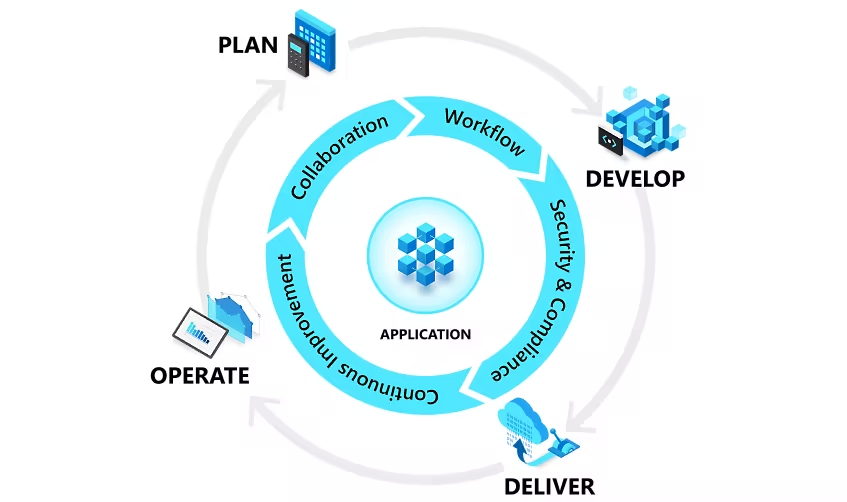
\includegraphics[width=0.9\linewidth]{images/EA/devops-lifecycle.png}
        \caption{DevOps-Lebenszyklus \\ \cite{EA:Web37}}
        \label{fig:devops-lifecycle}
    \end{figure}
      
    In Abbildung \ref{fig:devops-lifecycle} wird dargestellt, wie der DevOps-Lebenszyklus aussieht.
    Der Prozess \textbf{beginnt mit der Planung}. Dabei wird festgelegt, welche Funktionalitäten im nächsten Sprint umgesetzt werden sollen, um Kund/innen einen Mehrwert zu bieten. Hierbei wird auf \textbf{agiles Projektmanagement} gesetzt, um auf das Feedback der Anwender/innen einzugehen und falls gewünscht, entsprechende Änderungen vorzunehmen.
    
    Nachdem die Planung abgeschlossen ist, kann mit der \textbf{Entwicklung} begonnen werden. Neben der Implementierung neuer Funktionalitäten und der Behebung von Bugs wird der geschriebene Code auch getestet (siehe Kapitel \ref{}). Bevor eine neue Version der Software bereitgestellt wird, sollte diese vorher ausgiebig getestet werden. Dazu werden automatische Tests durchlaufen und anschließend kann die Software automatisch ausgeliefert werden. Realisiert wird dies mithilfe von CI/CD\footnote{Continuous Integration and Continuous Delivery}, das im Anschluss kurz beschrieben wird. Eine genauere Beschreibung kann in Kapitel \ref{} gefunden werden.

    \clearpage

    Die nächste Phase befasst sich mit der \textbf{Bereitstellung}. Dabei sollen entsprechende Anwendungen zuverlässig in einer Produktionsumgebung bereitgestellt werden. Dazu gehört auch die Konfiguration und Verwaltung der Infrastruktur, was beispielsweise mit Infrastructure as Code (IaC) erreicht werden kann. Dies wird im Abschnitt \ref{IaC} näher beschrieben.

    Treten in der Produktionsumgebung keine Fehler auf, so kann die Software für die Nutzer/innen zugänglich gemacht werden. Diese Phase bezeichnet man als \textbf{Ausführungsphase}. Die Software wird dabei überwacht und im Falle eines Fehlers wird versucht, diesen zu beheben. 

    Dieser Prozess wiederholt sich und trägt dazu bei, dass das \textbf{DevOps-Team kontinuierlich dazulernt} und somit bessere Ergebnisse liefern kann.
    \cite{EA:Web35, EA:Web37}

    Damit einzelne Phasen automatisiert und optimiert werden können, gibt es verschiedene Möglichkeiten, die eingesetzt werden können.
    Eine davon ist CI/CD. Dabei handelt es sich um eine Kombination aus kontinuierlicher Integration (Continuous Integration) und kontinuierlicher Lieferung (Continuous Delivery). Dadurch wird neuer Code ausgeliefert, ohne diesen manuell bereitstellen zu müssen.

    Die \textbf{kontinuierliche Integration (CI)} sorgt dafür, dass der Code eines bestimmten Branches, in der Regel des main-Branches, bei jedem neuen Commit getestet wird, indem die Anwendung gebaut wird.

    \begin{figure}[H]
        \centering
        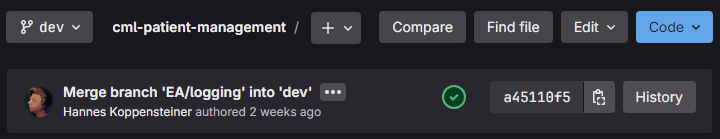
\includegraphics[width=1\linewidth]{images/EA/cml-ci-passed.png}
        \caption{Erfolgreicher Build - CGM MAXX LITE}
        \label{fig:cml-ci-passed}
    \end{figure}

    Abbildung \ref{fig:cml-ci-passed} zeigt einen Ausschnitt aus einem \textbf{GitLab-Repository}, das den erfolgreichen CI-Build eines Projekts dokumentiert.
    Im gezeigten Beispiel handelt es sich um den Microservice zur Verwaltung von Patientendaten. Sobald neue Änderungen am dev-Branch vorgenommen werden, wird versucht, die Anwendung zu bauen. In diesem Fall wurde Logging zur Anwendung hinzugefügt. Der grüne Haken auf der rechten Seite symbolisiert den erfolgreichen Build-Prozess.

    Sobald der CI-Prozess abgeschlossen ist, sorgt die \textbf{kontinuierliche Lieferung (CD)} dafür, dass die Software so vorbereitet wird, dass sie jederzeit bereitgestellt werden kann.
    \cite{EA:Web38}
    

    % --- I N F R A S T R U C T U R E   A S   C O D E ---    

    \subsubsection{Infrastructure as Code (IaC)} \label{IaC}

    Infrastructure as Code (IaC) ist eine \textbf{in DevOps angewandte Methode}, die insbesondere \textbf{in der kontinuierlichen Bereitstellung von Software Anwendung findet}. \\
    Dabei wird Code geschrieben, der es ermöglicht, die Infrastruktur automatisch zu konfigurieren und bereitzustellen, 
    sodass manuelle Eingriffe vermieden werden. \\
    \cite{EA:Web37}

    Diese Methode eignet sich daher besonders gut, um \textbf{komplexe und umfangreiche Umgebungen} bereitzustellen, die häufig aufgesetzt werden müssen. Dazu zählen unter anderem Entwicklungs- und Test-Umgebungen. \\
    \cite{EA:Web30, EA:Web39}
    
    IaC bietet dabei einige Vorteile:
    \begin{itemize}
        \item Umgebungen können einfach dupliziert werden
        \item Weniger Fehler durch automatische Erstellung
        \item Schnelle und zuverlässige Bereitstellung
    \end{itemize}

    Um Infrastruktur mithilfe von Code zu erzeugen, gibt es zwei verschiedene Ansätze:
    \begin{itemize}
        \item \textbf{Deklarativer Ansatz}
        \begin{itemize}[label=$\circ$]
            \item Der gewünschte Endzustand des Systems wird durch die \\ Definition von Ressourcen und deren Einstellungen beschrieben.
        \end{itemize}
        
        \item \textbf{Imperativer Ansatz}
        \begin{itemize}[label=$\circ$]
            \item Der gewünschte Endzustand wird durch die Beschreibung aller \\ notwendigen Schritte zur Konfiguration der Ressourcen erreicht.
        \end{itemize}
    \end{itemize}

    Damit die oben genannten Vorteile realisiert werden können, stehen zahlreiche Tools von verschiedenen Herstellern zur Verfügung. \cite{EA:Web40} \\
    Zu den bekanntesten IaC-Tools gehören: 
    \begin{itemize}
        \item Terraform
        \item AWS CloudFormation
        \item Ansible
    \end{itemize}

    Neben den genannten Tools existieren zahlreiche weitere Werkzeuge, die für die Erstellung und Verwaltung von Infrastruktur genutzt werden können.
     Da sich all diese Tools in bestimmten Punkten unterscheiden, ist es wichtig, ein für den Anwendungsfall passendes Werkzeug auszuwählen.

    Um die Unterschiede der genannten IaC-Tools zu verdeutlichen, werden diese in Tabelle \ref{tab:iac-tools} miteinander verglichen:

    \begin{table}[H]
        \centering
        \begin{tabular}{|l|c|c|c|}
        \hline
        \textbf{Kriterium} & \textbf{Terraform} & \textbf{CloudFormation} & \textbf{Ansible}\\ \hline
        Anbieter & HashiCorp & Amazon Web Services & Red Hat \\ \hline
        Ansatz & Deklarativ & Deklarativ & Deklarativ/imperativ \\ \hline
        Konfigurationssprache & HCL/JSON & YAML/JSON & YAML \\ \hline
        Multi-Provider-Support & Ja & Nein & Ja \\ \hline
        Kosten und Lizenzierung & Kostenlos & AWS-Ressourcen & Kostenlos \\ \hline
        \end{tabular}
        \caption{IaC-Tools}
        \label{tab:iac-tools}
    \end{table}

    Im weiteren Verlauf wird erklärt, wofür die einzelnen Tools verwendet werden, und wie sie sich in ihrer Funktionsweise unterscheiden.
    \cite{EA:Web41, EA:Web42, EA:Web43} \\


    % --- T E R R A F O R M ---
    
    \textbf{Terraform}

    Terraform ist ein von HashiCorp entwickeltes Tool für Infrastructure as Code (IaC), das die Bereitstellung und Verwaltung von Infrastruktur sowohl in Cloud-Umgebungen als auch On-Premise ermöglicht. Geschrieben werden die Konfigurationsdateien in der HashiCorp Configuration Language (HCL) oder in JSON, die beide eine simple und leicht verständliche Struktur aufweisen.
    
    Ein wesentlicher Vorteil von Terraform ist die Unterstützung zahlreicher \\Cloud-Dienstanbieter, darunter AWS, Azure und Google Cloud Platform. \\ \cite{EA:Web44}
    
    \begin{figure}[H]
        \centering
        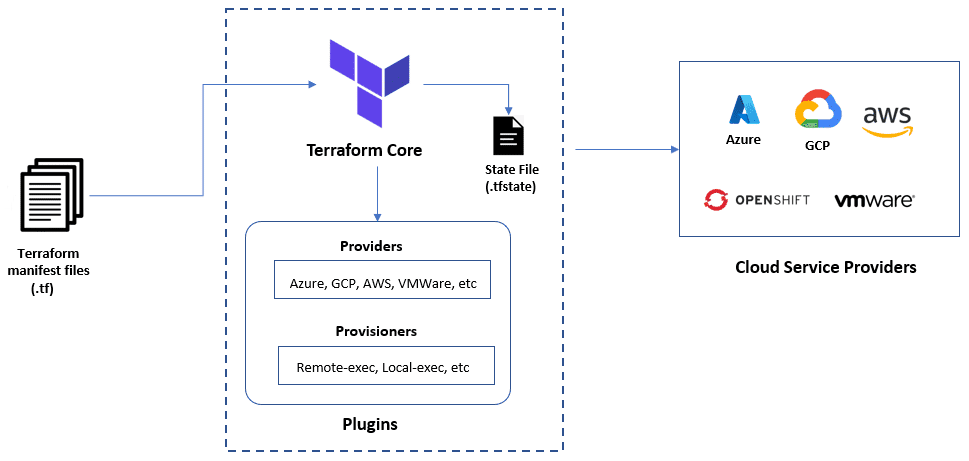
\includegraphics[width=1\linewidth]{images/EA/terraform-architecture.png}
        \caption{Terraform Architektur \\ \cite{EA:Web49}}
        \label{fig:terraform-architecture}
    \end{figure}

    Abbildung \ref{fig:terraform-architecture} veranschaulicht die grundlegende Architektur von Terraform.
    Der Prozess beginnt mit dem Erstellen einer Konfigurationsdatei, in der alle notwendigen Einstellungen vorgenommen werden, um den gewünschten Endzustand des Systems zu erreichen. Anschließend wird mithilfe der \textbf{Terraform CLI\footnote{Command-line Interface}} ein Ausführplan erstellt. Erst wenn dieser bestätigt wird, werden die Änderungen durchgeführt.

    Die Terraform CLI, auch Terraform Core genannt, ist das zentrale Werkzeug für die Verwaltung von Infrastruktur.
    Weiters interagiert sie mit \textbf{Providern}, die die Kommunikation mit unterschiedlichen Diensten ermöglichen. Dabei werden die vorliegenden Konfigurationen in die für den Dienstanbieter vorgesehenen API Calls umgewandelt und passen die Einstellungen entsprechend an. \\
    \cite{EA:Web44, EA:Web49}

    \clearpage

    % --- A W S   C L O U D F O R M A T I O N ---

    \textbf{AWS CloudFormation}

    Wie der Name bereits andeutet, handelt es sich um einen Dienst von Amazon Web Services, der speziell auf die \textbf{Bereitstellung von AWS-Ressourcen} ausgerichtet ist. Der Dienst selbst ist kostenlos. Es entstehen lediglich Kosten für die bereitgestellten Ressourcen, wie beispielsweise EC2-Instanzen.

    In Abbildung \ref{fig:aws-cloudformation} wird der Ablauf der Bereitstellung gezeigt:

    \begin{figure}[H]
        \centering
        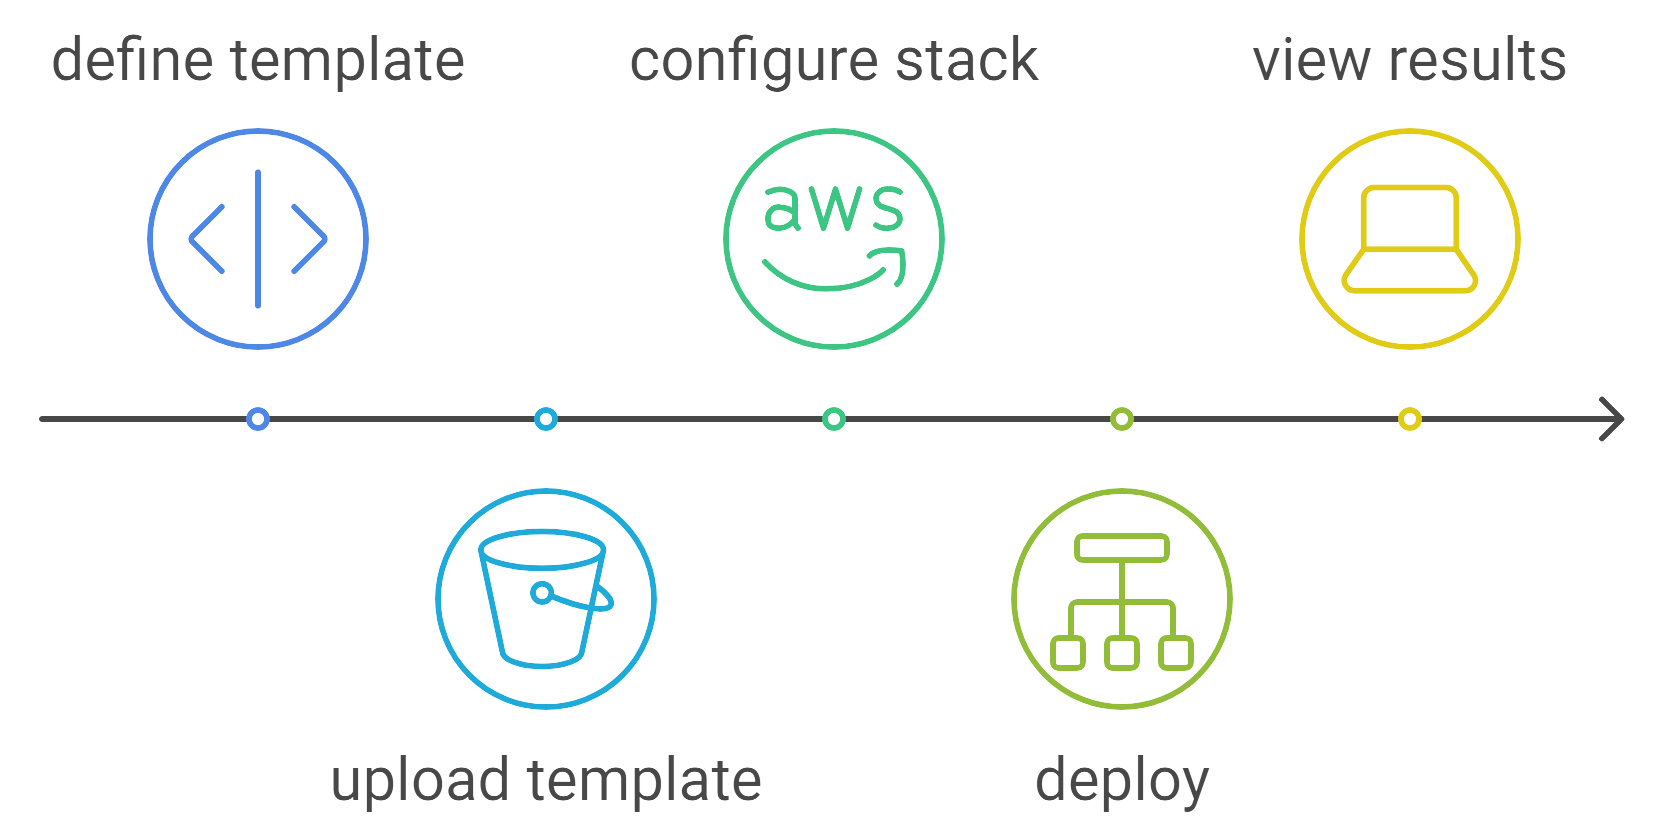
\includegraphics[width=0.7\linewidth]{images/EA/cloudformation-workflow.png}
        \caption{AWS CloudFormation Funktionsweise}
        \label{fig:aws-cloudformation}
    \end{figure}

    Ähnlich wie bei Terraform, muss auch bei CloudFormation eine \textbf{Vorlage} erstellt werden, welche die benötigten Ressourcen beschreibt.
    Bei der Konfigurationssprache kann entweder YAML oder JSON eingesetzt werden. Alle Ressourcen, die in einer Vorlage definiert werden, werden als eine Einheit betrachtet, die auch als \textbf{Stack} bezeichnet wird.

    Um die Änderungen einer Vorlage zu übernehmen, muss ein \textbf{Änderungssatz} erstellt werden. Dabei wird auf den Speicherort der ausgewählten Vorlage verwiesen, die entweder \textbf{lokal oder in einem Amazon S3-Bucket abgespeichert} werden kann. 
    Der Änderungssatz zeigt dabei, welche Änderungen vorgenommen werden und ähnelt somit einem Ausführungsplan in Terraform. 
    \cite{EA:Web50, EA:Web51}
    
    Der Unterschied zwischen diesen beiden Tools besteht darin, dass wenn in CloudFormation ein Fehler beim Änderungsvorgang auftritt, der Stack auf den letzten funktionsfähigen Stand zurückgesetzt wird. In Terraform hingegen werden nur die Ressourcen isoliert, die vom Fehler betroffen sind. Zudem unterstützt Terraform neue AWS-Funktionen oft schneller als CloudFormation selbst. 
    \cite{EA:Web52}

    \clearpage


    % --- R E D   H A T   A N S I B L E ---

    \textbf{Ansible}    

    Ansible ist kein IaC-Tool im eigentlichen Sinne. Es ist vielmehr ein Konfigurationswerkzeug, das sich auf die Automatisierung unterschiedlicher Tasks fokussiert. Dazu zählen unter anderem Systemupdates, die Installation von Software, das Einrichten einer Firewall, und vieles mehr. Um dies zu realisieren, werden sogenannte \textbf{Playbooks} eingesetzt, die in der Datenserialisierungssprache YAML geschrieben werden.

    Während Terraform besser für die Bereitstellung von Infrastruktur geeignet ist, spielt Ansible seine Stärken bei der Konfigurationsverwaltung aus. Beide Werkzeuge haben ihre Vor- und Nachteile. In der Praxis werden Terraform und Ansible häufig kombiniert, 
    um die Stärken beider Tools optimal zu nutzen.
    \cite{EA:Web45, EA:Web48}
    
    \begin{figure}[H]
        \centering
        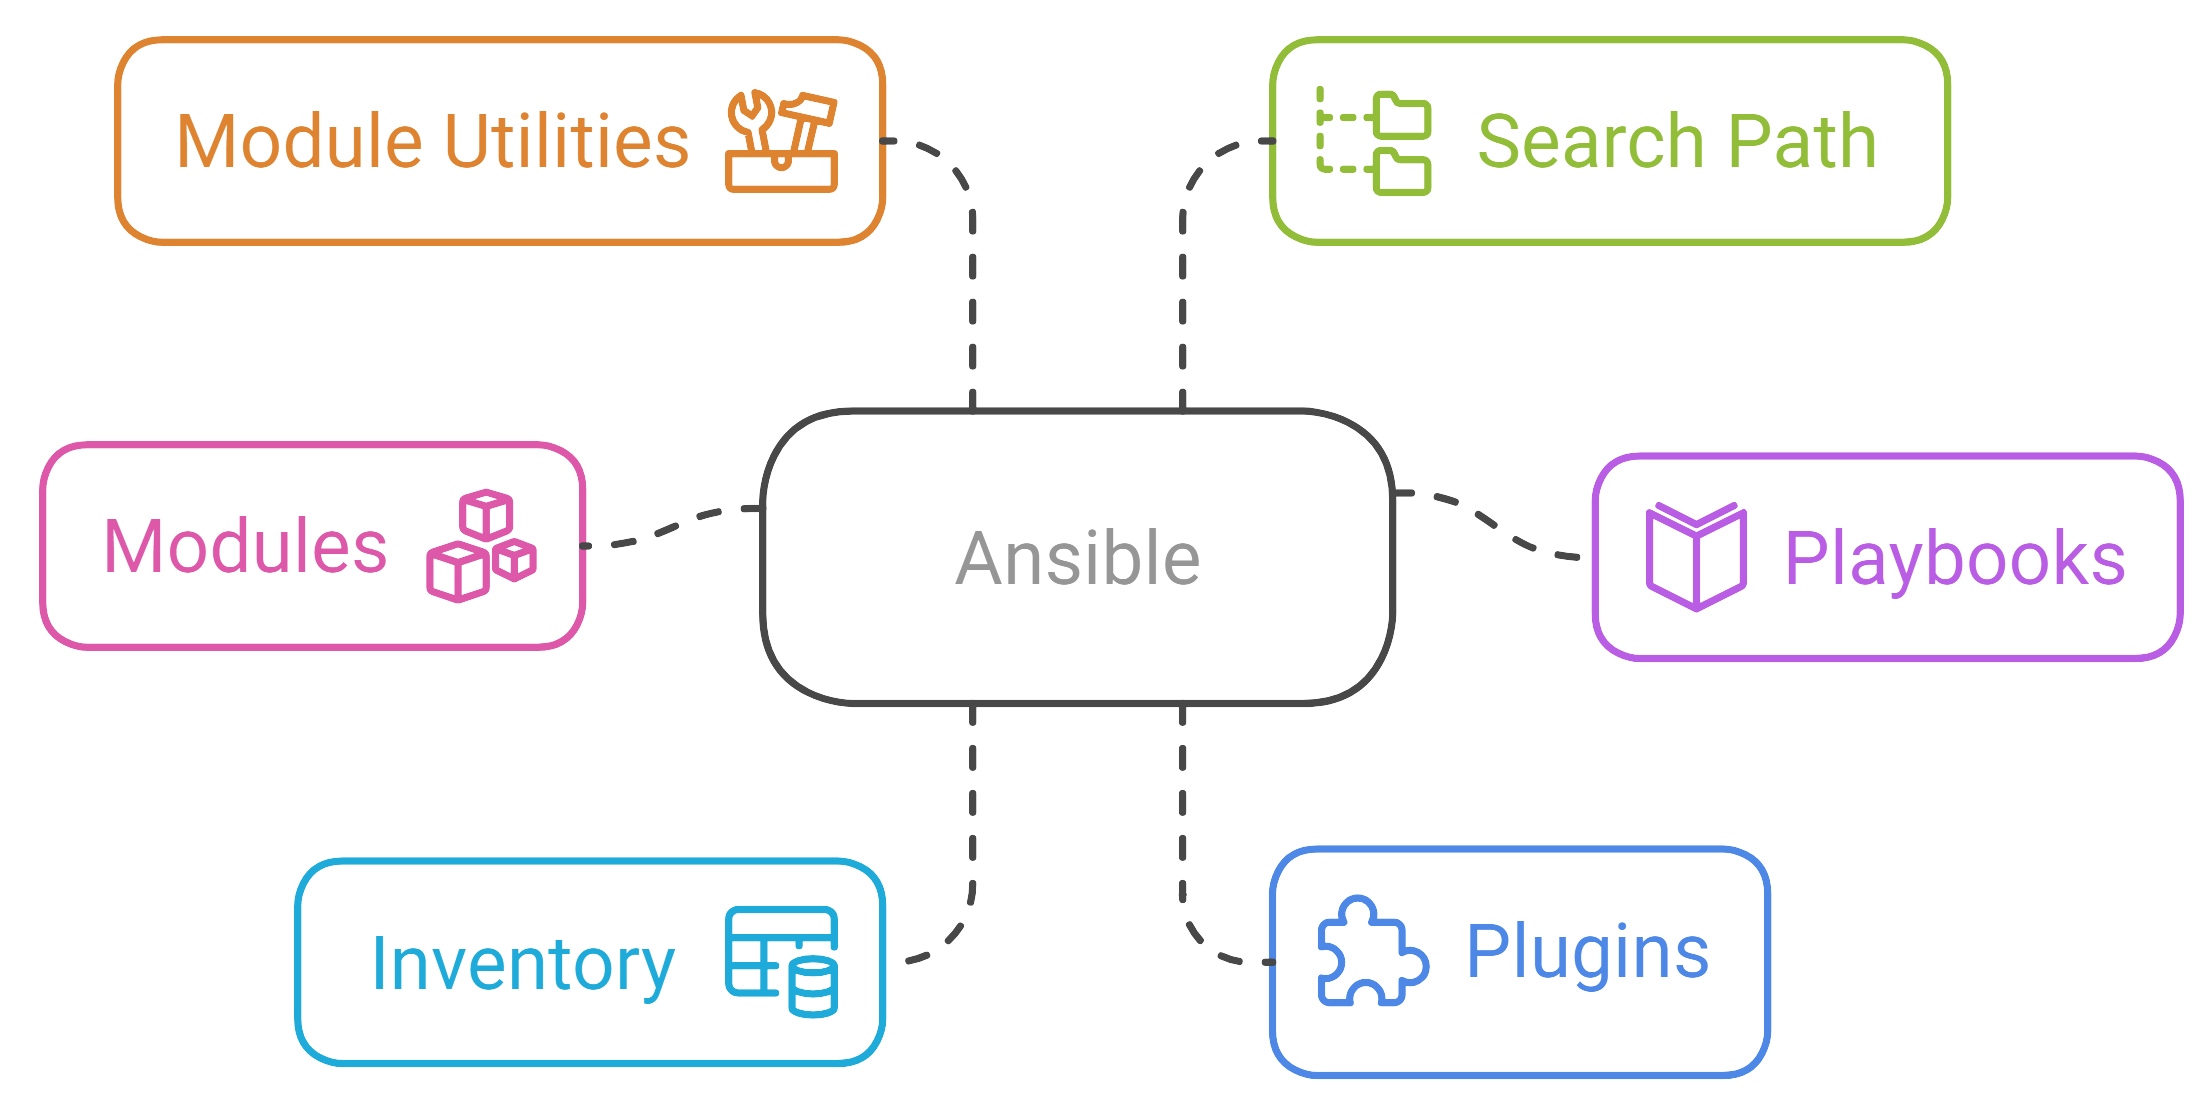
\includegraphics[width=0.7\linewidth]{images/EA/ansible-architecture.png}
        \caption{Ansible Architektur}
        \label{fig:ansible-architecture}
    \end{figure}

    Um die Funktionsweise von Ansible besser zu verstehen, wird die Architektur anhand der Grafik in Abbildung \ref{fig:ansible-architecture} näher erklärt. Diese setzt sich aus folgenden Komponenten zusammen:

    \begin{itemize}
        \item \textbf{Modules}
        \begin{itemize}[label=$\circ$]
            \item Skripte, die auf Managed Nodes\footnote{Geräte, die von Ansible verwaltet werden} kopiert und dort ausgeführt werden
            \item Standardmäßig erfolgt die Ausführung über SSH
            \item Erledigen die in den Playbooks definierten Tasks
        \end{itemize}
        
        \item \textbf{Module Utilities}
        \begin{itemize}[label=$\circ$]
            \item Mehrfach vorkommende identische Codeausschnitte werden gespeichert
            \item Redundanter Code wird vermieden und die Wartung wird erleichtert
        \end{itemize}
        
        \item \textbf{Plugins}
        \begin{itemize}[label=$\circ$]
            \item Ergänzt Ansible um neue Funktionen
            \item Eigene Plugins können mithilfe von Python geschrieben werden
        \end{itemize}
        
        \item \textbf{Playbooks}
        \begin{itemize}[label=$\circ$]
            \item YAML-Dateien für die Konfiguration von Managed Nodes
            \item Einfach zu lesen
        \end{itemize}
        
        \item \textbf{Inventory}
        \begin{itemize}[label=$\circ$]
            \item Liste mit den Managed Nodes, die durch Ansible verwaltet werden
            \item Gruppierung von Hostnamen und IP-Adressen möglich
            
        \end{itemize}
        
        \item \textbf{Search Path}
        \begin{itemize}[label=$\circ$]
            \item Gibt an, wo benötigte Module, Plugins, Playbooks, usw. zu finden sind
        \end{itemize}
        
    \end{itemize}
    \cite{EA:Web46, EA:Web47} \\


    % --- I N F R A S T R U C T U R E   A S   C O D E   -   A B S C H L U S S ---

    Abschließend lässt sich sagen, dass es nicht das eine \glqq{perfekte}\grqq\ Werkzeug gibt. 
    Daher ist es wichtig, den genauen Anwendungsfall zu kennen, um auf dieser Grundlage ein passendes Tool auszuwählen.
    Das Ziel sollte sein, eine einfache und schnelle Lösung zu finden, um Infrastruktur und/oder Software bereitzustellen und so einen Wettbewerbsvorteil zu erzielen.

    Zudem wird der Entwicklungsprozess erleichtert, da durch die einfache Reproduzierbarkeit von Systemen weniger Fehler auftreten.
    Auf diese Weise können sich die Entwickler/innen auf ihre eigentlichen Aufgaben konzentrieren, ohne stundenlang nach der Ursache eines Fehlers suchen zu müssen.